\subsection{Resultados}

\begin{figure}[H]
\begin{center}
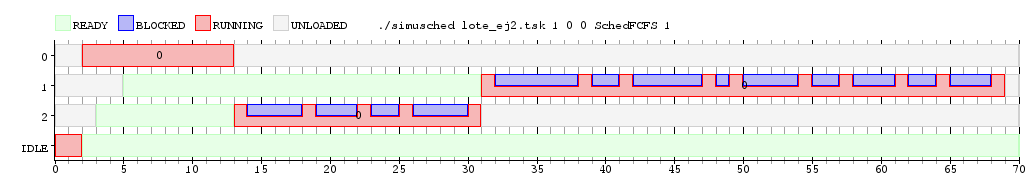
\includegraphics[width=1.1\textwidth]{img/ej2_1.png}
     \caption{FCFS con 1 núcleo}
\end{center}
\end{figure}

\textbf{Conclusiones:} Se puede ver claramente que se ejecutan las tareas de forma FCFS, es decir primero se ejecuta el proceso 0 ya que es el primero en llegar (2 unidades de tiempo) una vez finalizado se pasa la ejecucion al proceso 2 (que llego en 3 unidades de tiempo), este ejecuta las 4 llamadas bloquenates y finalmente se pasa la ejecucion al proceso 1 que fue el ultimo en llegar (5 unidades de tiempo) ejecutando las 9 llamadas bloquentes. Tambien se puede ver a simple vista que las llamadas bloqueantes, respetan el bmin y bmax


\begin{figure}[H]
\begin{center}
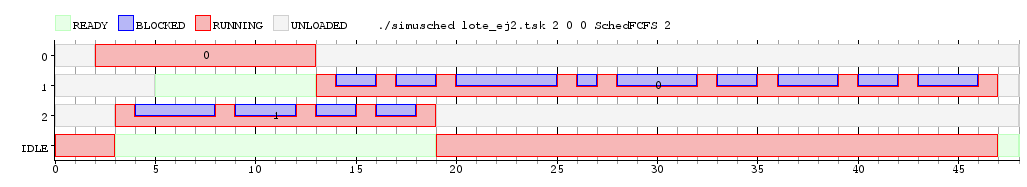
\includegraphics[width=1.1\textwidth]{img/ej2_2.png}
     \caption{FCFS con 2 núcleos}
\end{center}
\end{figure}

\textbf{Conclusiones:} En este experimento se puede ver que el funcionamiento es similar al experimento anterior, la única diferencia es que mientras se ejecuta el proceso 0, es decir cuando llega el proceso 2, al haber dos núcleos este no espera a la finalizacion del proceso 0 sino que arranca directamente su ejecución en el otro núcleo. Finalmente el proceso 1 (el restante) se ejecuta en el núcleo 0 cuando el proceso 0 (que es el primero en terminar) termina (es decir, se libera un núcleo).


\begin{figure}[H]
\begin{center}
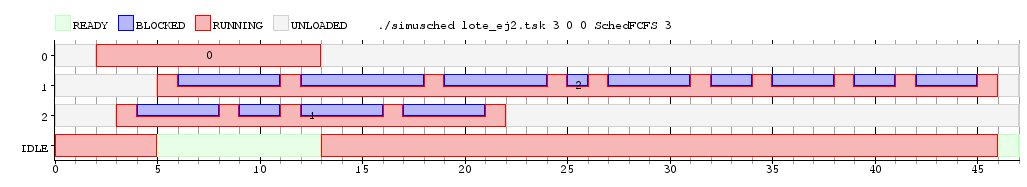
\includegraphics[width=1.1\textwidth]{img/ej2_3.png}
     \caption{FCFS con 3 núcleos}
\end{center}
\end{figure}

\textbf{Conclusiones:} Idéntico al caso anterior, pero con diferencia de que ahora tenemos tres núcleos y, por lo tanto, al haber solo 3 procesos, ninguna tiene que esperar a que otro termine, ya que cada uno puede correr en un núcleo distinto. Es por ese motivo que cada proceso se ejecuta en el instante en que llega.












